The architecture of a network is defined by the number of the units the it has and how they are 
connected to each other. A group of units that works in linear combinations is called \textbf{layer}, 
most of architecture arrange these layers in a chain structure in which each layer is a function of the
layer that preceded it. 
\newline 
In this structure, the first layer is given by $\mathbf{h}^{(1)} = g^{(1)} \left( \mathbf{W}^{(1)\top}
\mathbf{x} + \mathbf{b}^{(1)} \right)$ and the second layer is given by $\mathbf{h}^{(2)} = g^{(2)} 
\left( \mathbf{W}^{(2)\top} \mathbf{h}^{(1)} + \mathbf{b}^{(2)} \right)$ and so on. This mean that in 
this chain-based architectures, the main architectural considerations are choosing the depth of the 
network and the width of each layer. Generally speaking, one hidden layer is sufficient to fit the
training set, but it isn't as optimized as a deeper network. The ideal network architecture for a task
must be found via experimentation with the validation set error.

\subsection{Universal Approximation Properties and Depth}
Feedforward networks with hidden layers provide a universal approximation framework:
\begin{theorem}[Universal Approximation Theorem]
For any continuous $f$ on a closed and bounded region of $\mathbb{R}^d$ and any tolerance 
$\varepsilon > 0$, there is a network with \textbf{one hidden layer} of $N$ units and a linear output,
$$\hat{f}(\boldsymbol{x}) = \sum_{i=1}^{N} v_i \, g\left(\boldsymbol{w}_i^\top \boldsymbol{x} + 
b_i\right),$$ with $|f(\boldsymbol{x}) - \hat{f}(\boldsymbol{x})| < \varepsilon$ for every 
$\boldsymbol{x}$ in the region. Valid for sigmoid, tanh, ReLU: any continuous $g$ that is not a polynomial.
\end{theorem}
In other words, one hidden layer can represent any continuous function as accurately as we want.
\newline
This theorem means that regardless of what function we are trying to learn, we know that a large MLP 
will be able to represent it. We are not guaranteed that the training algorithm will be able to learn
that function.

\subsubsection{Sigmoid Application of Universal Approximation Theorem}
A hidden unit with one input computes $\sigma(wx + b) = \sigma(k(x - a))$ where $k = w$ is the 
\textbf{weight} that sets the steepness and $ a = -\frac{b}{w}$ is the bias that describe where the 
step happens.
\newline
In Fig \ref{fig:step_sigmoid} it is shown that a large weight turns the sigmoid into a \textbf{step}.
\begin{figure}[H]
    \centering
    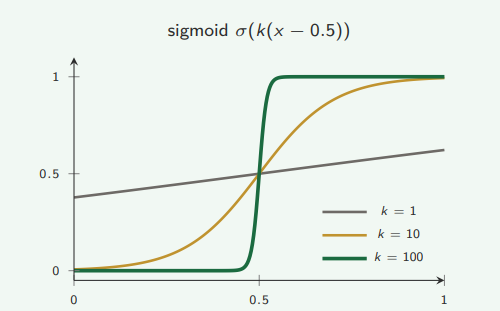
\includegraphics[width=0.35\linewidth]{immagini/step_sigmoid.png} 
    \caption{Steep sigmoid}
    \label{fig:step_sigmoid}
\end{figure}
If we take a network with one input and two hidden sigmoid, each unit is a \textbf{soft step} and their
difference is a \textbf{bump} (Fig \ref{fig:bump_sigmoid}).
\begin{figure}[H]
    \centering
    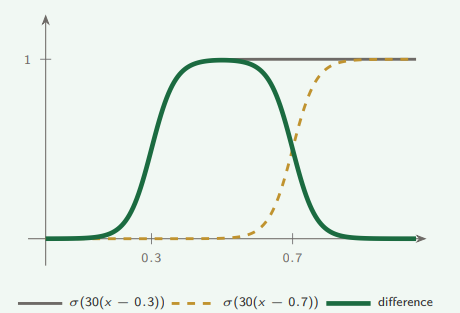
\includegraphics[width=0.35\linewidth]{immagini/bump_sigmoid.png} 
    \caption{Two sigmoid units build a bump}
    \label{fig:bump_sigmoid}
\end{figure}
\noindent
So in conclusion the approximation can be done with the sums of bumps, the recipe is:
\begin{enumerate}
    \item Split [0,1] into N intervals of width 1/N
    \item Put a bump of height $h_i = f(interval\ centre)\ \forall\ interval\ i$
    \item Add the bumps
\end{enumerate}
So formally in the network:
\begin{equation}
    \hat{f}(x) = h_1 + \sum_{i=2}^{N} (h_i - h_{i-1}) \, \sigma(k(x - a_i))
\end{equation}
As we can see steps are shared within the bumps(Fig \ref{fig:curve_sigmoid}), so the sum needs only $N - 1$ sigmoid unit plus 
a bias.
\begin{figure}[H]
    \centering
    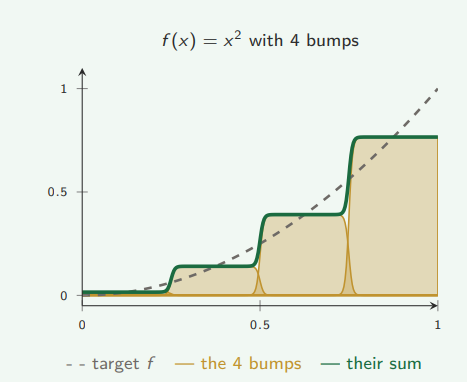
\includegraphics[width=0.35\linewidth]{immagini/network_curve_sigmoid.png} 
    \caption{Two sigmoid units build a bump}
    \label{fig:curve_sigmoid}
\end{figure}
\noindent
The approximation is corrected then by modifying the number of units and the parameters, in 
Fig \ref{fig:smooth_curve} we can see that with a moderate k the steps overlap and the sum becomes
a smooth curve.
\begin{figure}[H]
    \centering
    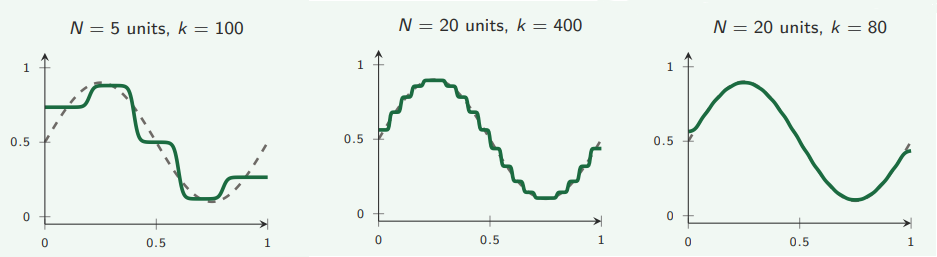
\includegraphics[width=0.7\linewidth]{immagini/smooth_curve.png} 
    \caption{Smooth curve evolution}
    \label{fig:smooth_curve}
\end{figure}
\noindent
By the same logic we can also represent \textbf{Peak} and \textbf{Kink} (Fig \ref{fig:peak_kink})
\begin{figure}[H]
    \centering
    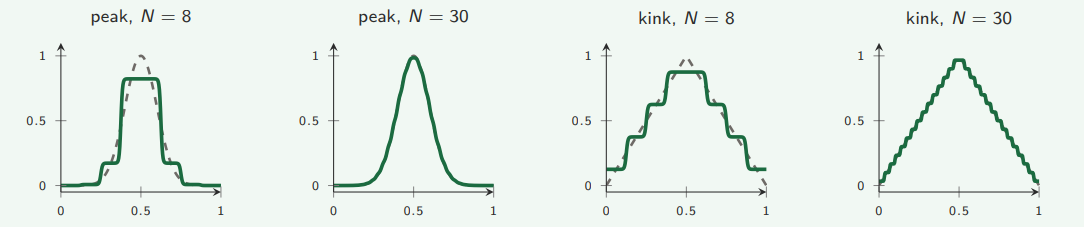
\includegraphics[width=0.99\linewidth]{immagini/peak_kink_sigmoid.png} 
    \caption{Peak and Kink evolution}
    \label{fig:peak_kink}
\end{figure}
\noindent
For the case of \textbf{Jumps} when the function is discontinuos, the bigger is k and the narrower the
zone of the error is, but it is never zero for definition, because the sum of sigmoid is continuous as 
shown in Fig \ref{fig:jump_sigmoid}
\begin{figure}[H]
    \centering
    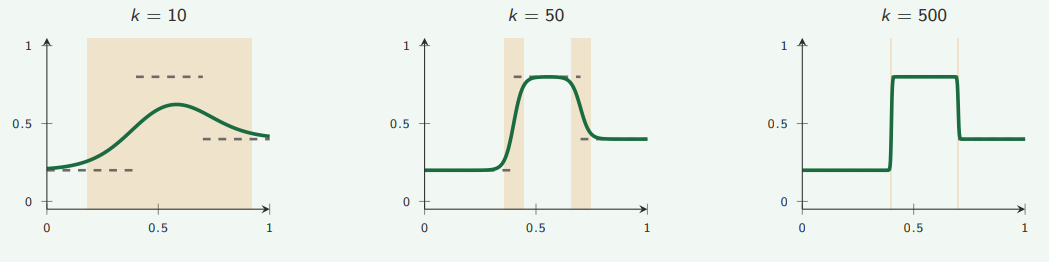
\includegraphics[width=0.99\linewidth]{immagini/jump_sigmoid.png} 
    \caption{Jump approximation}
    \label{fig:jump_sigmoid}
\end{figure}

\subsubsection{ReLU Application of Universal Approximation Theorem}
The foundational principle for function approximation with ReLU remains equivalent to the sigmoid 
case: decomposing the input space and summing elementary local building blocks to construct the 
target function. However, the geometric properties of these building blocks differ due to the 
piecewise linear nature of this function. Unlike the sigmoid function, which generates smooth steps and 
bell-shaped curves, a single hidden unit with ReLU computes a linear \textbf{ramp}:
\begin{equation}
h(x) = \max\left(0, w x + b\right)
\end{equation}
where the weight $w$ controls the slope and the bias $b$ determines the activation threshold (the elbow point).
\begin{itemize}
\item Subtracting \textbf{three} shifted ReLU units with opposite slopes yields a \textbf{triangular bump} (tent function).
\item Summing these triangular bumps creates a piecewise linear spline that fits any continuous 1D target function.
\end{itemize}

\begin{figure}[H]
    \centering
    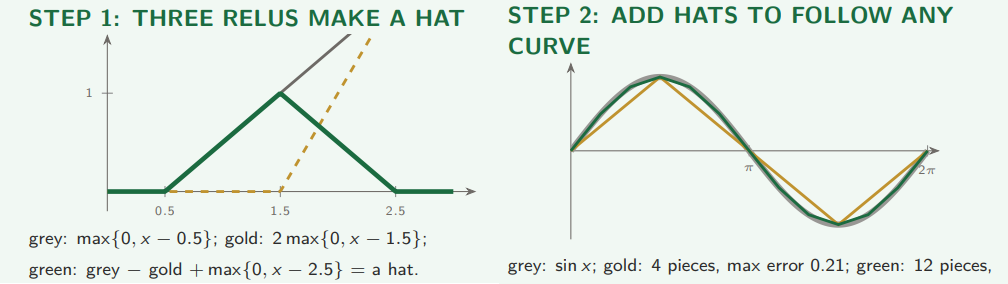
\includegraphics[width=0.99\linewidth]{immagini/relu_curve.png} 
    \caption{Approximation with ReLU}
    \label{fig:relu_curve}
\end{figure}

\subsubsection{Two-dimensional approximation}
In one dimension, a sigmoid unit produces a smooth step. In two dimensions, the same unit
\[
    h(\mathbf{x})=\sigma(w_1x_1+w_2x_2+b)=\sigma(\mathbf{w}^\top\mathbf{x}+b),
    \qquad \sigma(z)=\frac{1}{1+e^{-z}},
\]
with input $\mathbf{x}=(x_1,x_2)$, can be seen as that step stretched along the new dimension. 
Plotted over the $(x_1,x_2)$ plane, it gives a surface that is low on one side of a line and high on
 the other. We call this surface a \textbf{wall}.
The unit depends on $\mathbf{x}$ only through the scalar $\mathbf{w}^\top\mathbf{x}+b$, so $h$ is 
constant on every line
\[
    w_1x_1+w_2x_2+b=c .
\]
Indeed, if we move by a small displacement $(\Delta x_1,\Delta x_2)$ along such a line, the quantity 
$\mathbf{w}^\top\mathbf{x}+b$ does not change, hence $\mathbf{w}^\top\Delta\mathbf{x}=0$. This means 
that \emph{the level lines are perpendicular to $\mathbf{w}$}, and $\mathbf{w}$ points in the 
direction in which $h$ grows fastest, i.e.\ the direction in which the wall rises.
The parameters play the following roles:
\begin{itemize}
    \item The \textbf{direction} of $\mathbf{w}$ sets the orientation of the wall. For example, $\mathbf{w}=(1,0)$ gives vertical level lines, $\mathbf{w}=(0,1)$ gives horizontal ones, and $\mathbf{w}=(1,1)$ gives diagonal lines $x_1+x_2=\text{const}$.
    \item The \textbf{norm} $\|\mathbf{w}\|$ sets the steepness: large weights give a nearly vertical transition, small weights a gentle one.
    \item The \textbf{bias} $b$ translates the wall without changing its orientation. The transition, where $h=1/2$, lies on the line $\mathbf{w}^\top\mathbf{x}+b=0$.
\end{itemize}
The problem with a wall is that it is infinitely long along the direction in which $h$ does not 
change, so it cannot be a localized bump. To enclose a bounded region we need to combine several 
walls with \emph{different orientations}: the result is a \textbf{tower}.
A concrete construction for the square $[-1,1]^2$ uses four hidden units with steepness $k$:
\[
    s(\mathbf{x})=\sigma\big(k(x_1+1)\big)+\sigma\big(-k(x_1-1)\big)+\sigma\big(k(x_2+1)\big)+\sigma\big(-k(x_2-1)\big).
\]
For large $k$, $s\approx 4$ inside the square, $s\approx 3$ outside it but beyond a single side, and $s\approx 2$ in the outer corner regions. Summing the walls alone therefore does not give a uniform plateau. Adding an output unit that thresholds the sum,
\[
    T(\mathbf{x})=\sigma\big(k\,(s(\mathbf{x})-3.5)\big),
\]
yields $T\approx 1$ inside the square and $T\approx 0$ elsewhere, which is a tower. This construction
uses five units arranged in two layers, since the second nonlinearity is what produces the flat top. 
With a single hidden layer and a linear readout, a tower can still be approximated, but with more 
units, for example by combining wall pairs in various positions.
This approach has a price. To approximate an arbitrary function, we can cover the input space with a 
grid, cutting each of the $d$ axes into $n$ pieces and placing one tower per cell. This requires 
$n^d$ towers, so the number of units grows exponentially with the input dimension.
\begin{figure}[H]
    \centering
    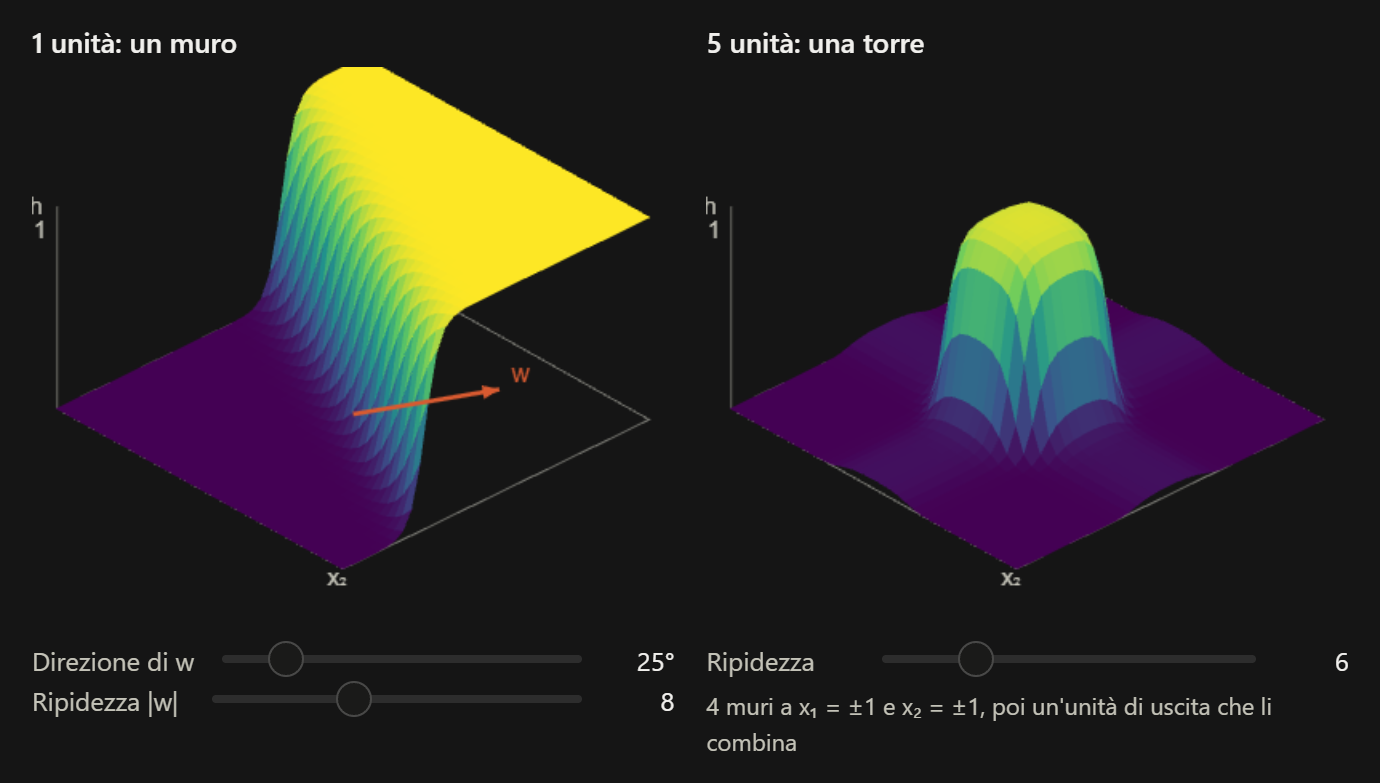
\includegraphics[width=0.99\linewidth]{immagini/wall_tower_curve.png}
    \caption{3d surface plot}
    \label{fig:wall_tower_curve}
\end{figure}

\subsection{Two sigmoid units in 2D}
to build intuition for the tower construction above, we have to explain how two sigmoid units combine
together to define a partially bounded region (two units are never enough to enclose a region). 
First of all, each unit cuts the plane (Fig \ref{fig:plane_cutted}): $\sigma{(w_1x_1 + w_2x_2 + b)}$ is:
\begin{itemize}
    \item 0.5 on the line $w_1x_1 + w_2x_2 + b = 0$
    \item <0.5 on one side and near to 0 far from the line (the unit goes off)
    \item >0.5 on the other side and near to 1 far from the line (the unit is on)
\end{itemize}
\begin{figure}[H]
    \centering
    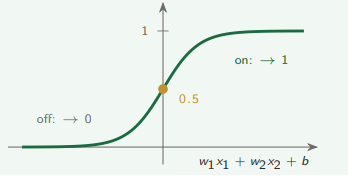
\includegraphics[width=0.5\linewidth]{immagini/plane_cutted.png}
    \caption{sigmoid unit}
    \label{fig:plane_cutted}
\end{figure}
\begin{figure}[H]
    \centering
    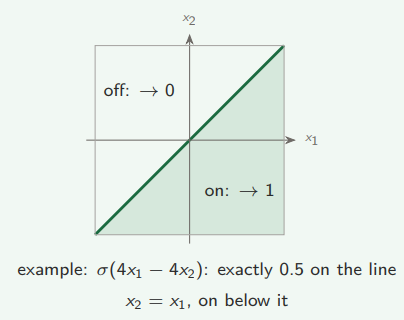
\includegraphics[width=0.5\linewidth]{immagini/two_regions.png}
    \caption{sigmoid unit}
    \label{fig:two_regions}
\end{figure}
\noindent
So computing the output ($\hat{y} = v_AA + v_bB$) by combinating two hidden units we can find three 
types of combination: \textit{Band, Curved Corner and Wedge}. 
\newline
\textbf{DA SPOSTARE}
The final network output $\hat{y} = \sum_{i} v_i h_i$ represents a continuous score rather than 
a probability. Classification is achieved by comparing this score against a decision threshold 
(e.g., $0.5$ for a band or wedge, and $1.5$ for a corner). Consequently, the output layer's bias 
acts as the negative of this threshold, satisfying the condition $\text{bias} = -\text{threshold}$.
\textbf{DA SPOSTARE}
\subsubsection{Band}
The band is obtained when both units ignore one of the two inputs, the bias indicate where the
lines are, the band comes out by the final weights that are opposed $v_A = -v_B$.
In Fig \ref{fig:band_nn} $x_2$ has weight 0 so in the 2D-space of the input the sigmods are two 
vertical lines (Fig \ref{fig:band}) and the score $\hat{y}$ is shown in Fig \ref{fig:band_score}. 
\begin{figure}[H]
    \centering
    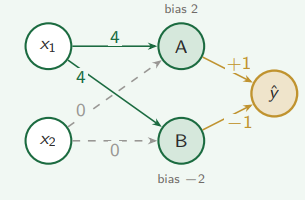
\includegraphics[width=0.5\linewidth]{immagini/band_nn.png}
    \caption{Band threshold = 0.5}
    \label{fig:band_nn}
\end{figure}
\begin{figure}[H]
    \centering
    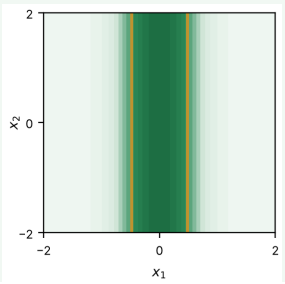
\includegraphics[width=0.5\linewidth]{immagini/band.png}
    \caption{Band $\sigma{(4x_1 + 2)} - \sigma{(4x_1 - 2)}$}
    \label{fig:band}
\end{figure}
\begin{figure}[H]
    \centering
    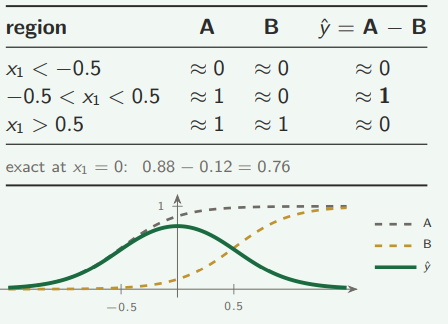
\includegraphics[width=0.5\linewidth]{immagini/band_score.png}
    \caption{Cross section along $x_1$ with the 1D bump}
    \label{fig:band_score}
\end{figure}

\subsubsection{Curved Corner}
The curved corner happens when we add the two crossing lines at the origin that split the plane into 
four sector, as shown in Fig \ref{fig:curved_corner}. Here the decision threshold is 1.5 because we
predict 1 when both units are on (right sector). It's \textit{curved} because in the origin 
$\hat{y} = 1 < 1.5$
\begin{figure}[H]
    \centering
    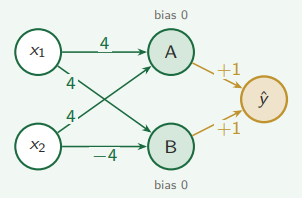
\includegraphics[width=0.5\linewidth]{immagini/curved_corner_nn.png}
    \caption{Curved Corner threshold 1.5}
    \label{fig:curved_corner_nn}
\end{figure}
\begin{figure}[H]
    \centering
    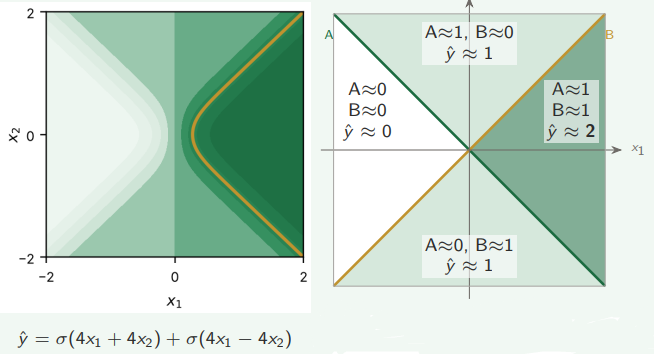
\includegraphics[width=0.5\linewidth]{immagini/curved_corner.png}
    \caption{Curved Corner}
    \label{fig:curved_corner}
\end{figure}

\subsubsection{Wedge}
The wedge is similar to the curved corner, the difference is on the hidden units weigth as shown in
Fig \ref{fig:wedge_nn} infact here the two lines are subtracted (threshold 0.5)
\begin{figure}[H]
    \centering
    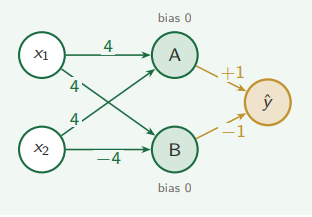
\includegraphics[width=0.5\linewidth]{immagini/wedge_nn.png}
    \caption{Wedge in the nn}
    \label{fig:wedge_nn}
\end{figure}
\begin{figure}[H]
    \centering
    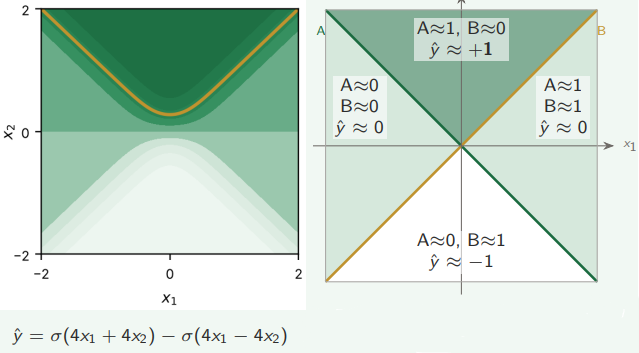
\includegraphics[width=0.5\linewidth]{immagini/wedge.png}
    \caption{Wedge}
    \label{fig:wedge}
\end{figure}

\subsection{Deep vs Shallow}
We said that a network with a single layer is sufficient to represent any function, but the layer may 
be infeasibly large. In many circumstances, using deeper models can reduce the number of units 
required to represent the desired function and can reduce the amount of generalization error.
\begin{definition}[The Exponential Capacity of Depth]
A ReLU network with $d$ inputs, $L$ layers of $q$ units can split the input space into about
$$\left(\frac{q}{d}\right)^{d(L-1)} q^d$$
linear regions: exponential in the depth $L$.
\end{definition}
For example in Figure \ref{fig:composition_relu} we see that with $t(x) = 2max{0,x} - 4max{0,x - \frac{1}{2}}$
two ReLUs make a tent on [0,1], $t(t(x))$ \textbf{folds} the tent into two tents and so on.
\begin{figure}[H]
    \centering
    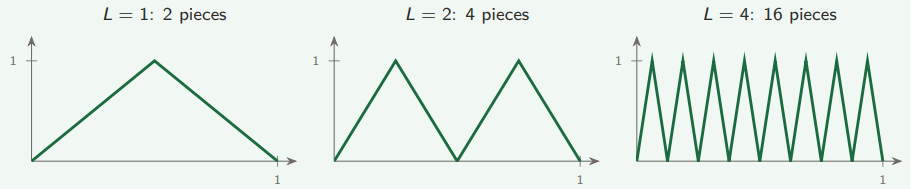
\includegraphics[width=0.7\linewidth]{immagini/composition_relu.png}
    \caption{Exponential advange of deeper rectifier networks}
    \label{fig:composition_relu}
\end{figure}
\noindent
Figure \ref{fig:space_fold} shows a geometric representation of this concept, an absolute value unit 
$g(z) = |z|$ gives the same output for a point and its mirror image across the line z = 0, it folds 
the plane like a sheet of paper. Whatever the next layers compute is repeated on both halves; 
each further layer folds again: 2, 4, 8, . . . copies.
\begin{figure}[H]
    \centering
    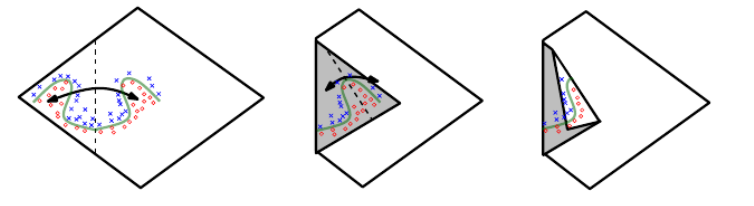
\includegraphics[width=0.6\linewidth]{immagini/space_fold.png}
    \caption{Exponential advantage of deeper rectifier networks}
    \label{fig:space_fold}
\end{figure}
\noindent
A deep model assumes that the target is a composition of simpler functions or has a repeated structure,
using the fold concept, depth can be exponentially more efficient. 